Se calcula sobre la representación en forma de onda del sonido computando una transformación discreta de Fourier ( una transformación discreta de Fourier consiste en la captura mediante ventanas triangulares en movimiento L de secciones de la onda , Fig. 4.3) trasladada a lo largo de la onda ( L ,2L, 3L ... )
\begin{center}
  \[
X(n, \omega) = \sum_{m=-\infty}^{\infty} x[m] \cdot w[m - n] \cdot e^{-j \omega m}
\]  
\end{center}
Donde:
\begin{itemize}
  \item \textbf{\[x[m]\]} Señal original de audio en tiempo discreto. P.ej: muestras digitales del sonido
  \item \textbf{\[m\]} Índice de la muestra para recorrer la señal punto a punto.
  \item \[w[m - n]\] Ventana aplicada sobre la señal al rededor del instante \[n\].
  \item \[n\] Posición temporal de la ventana.
  \item \[\cdot e^{-j \omega m}\] Onda compleja usada para medir la presencia de una frecuencia concreta. \[j\] es la unidad imaginaria, \[w\] es la frecuencia angular digital.
\end{itemize}
Cada celda ( ventana ) de la transformada es compleja ( contiene magnitud y fase ) y la transformada en general es invertible, por lo que se puede obtener la onda inicial a partir de la representación.

\begin{figure}[H]
    \begin{center}
    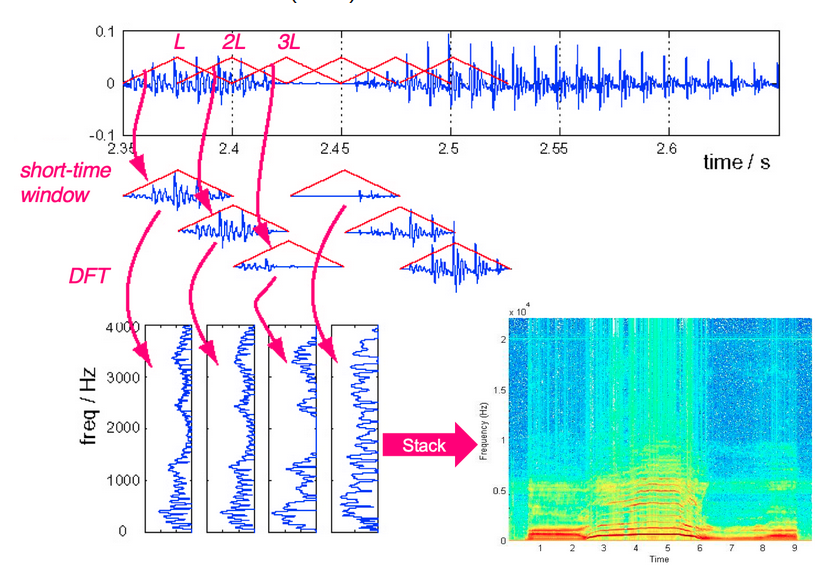
\includegraphics[width=0.7\textwidth]{commons/Fig3.png}
    \caption{Proceso de computar una transformada en tiempo corto de Fourier a partir de una onda. Imagen de Bryan Pardo}
    \label{fig:STFT}
    \cite{rafii18}
    \end{center}
\end{figure}
Como parámetros importantes, presenta el tipo de ventana que utiliza ( gaussiana, rectangular , triangular, cuadrática ... ), la longitud de la ventana y la distancia entre ventanas adyacentes.




